\section{Einleitung}
Ziel der Arbeit im Rahmen der Vorlesung Robotik war es, das Spiel \glqq Vier Gewinnt\grqq ~auf einer LED-Matrix zu implementieren und eine Künstliche Intelligenz zu entwickeln, die es ermöglicht auch alleine das Spiel zu nutzen.

\section{Vier Gewinnt}
\label{sec:vierg}
Bei \glqq Vier Gewinnt\grqq ~handelt es sich um ein Spiel, bei dem zwei Spieler auf einem klassischerweise 6x7 Feld (6 Zeilen, 7 Spalten) versuchen über das jeweilige Setzen von Steinen eine Reihe von vier Steinen zu erzeugen. Die Vorraussetzungen dabei sind, dass der jeweilige Stein am unteren Ende der Spalte gesetzt wird und die Spieler stets nacheinander am Zuge sind.

\begin{figure}[!hbt]
	\centering
	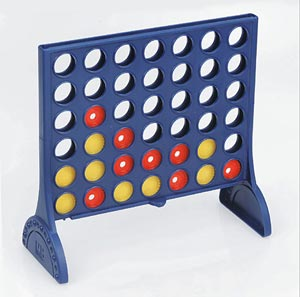
\includegraphics[scale=0.8]{4Gewinnt.jpeg}
	\caption{Ein klassisches Vier-Gewinnt-Spiel}
\end{figure}

Aus mathematischer Sicht ist \glqq Vier Gewinnt\grqq ~ein Spiel mit perfekter Information. Dies bedeutet, dass zu jedem Zeitpunkt alle vorhergehenden Züge bekannt sind. Diese perfekte Information sorgt dafür, dass das Spiel vollständig gelöst ist. Daraus kann abgeleitet werden, dass der Ausgang des Spiels für zwei perfekt spielende Gegner davon abhängig ist, in welche Spalte der erste Stein gesetzt worden ist: Wurde der erste Stein in die mittlere Spalte gesetzt, so gewinnt bei perfektem Spiel stets der erste Spieler. Beim Setzen in eine der Nachbarspalten, endet das Spiel unentschieden, sollte der erste Stein in eine der übrigen Spalten gesetzt werden, so gewinnt der zweite Spieler. 

\section{LED-Matrix und Darstellung des Spielfeldes}
Um \glqq Vier Gewinnt\grqq ~auf einer LED-Matrix abbilden zu können müssen zwei wesentliche Eigenschaften von der Matrix erfüllt werden: Zunächst muss die Matrix eine Mindestgröße von 6x7 besitzen, zum anderen muss sie fähig sein mindestens zwei unterschiedliche Farben abzubilden.
Bei der Suche nach einer geeigneten Matrix hat sich herausgestellt, dass vor allem die zweite Eigenschaft ein Problem darstellt.
Es konnte dennoch eine geeignete Matrix gefunden werden:
Das \glqq Adafruit 16x32 RGB LED matrix panel\grqq.

\begin{figure}[!hbt]
	\centering
	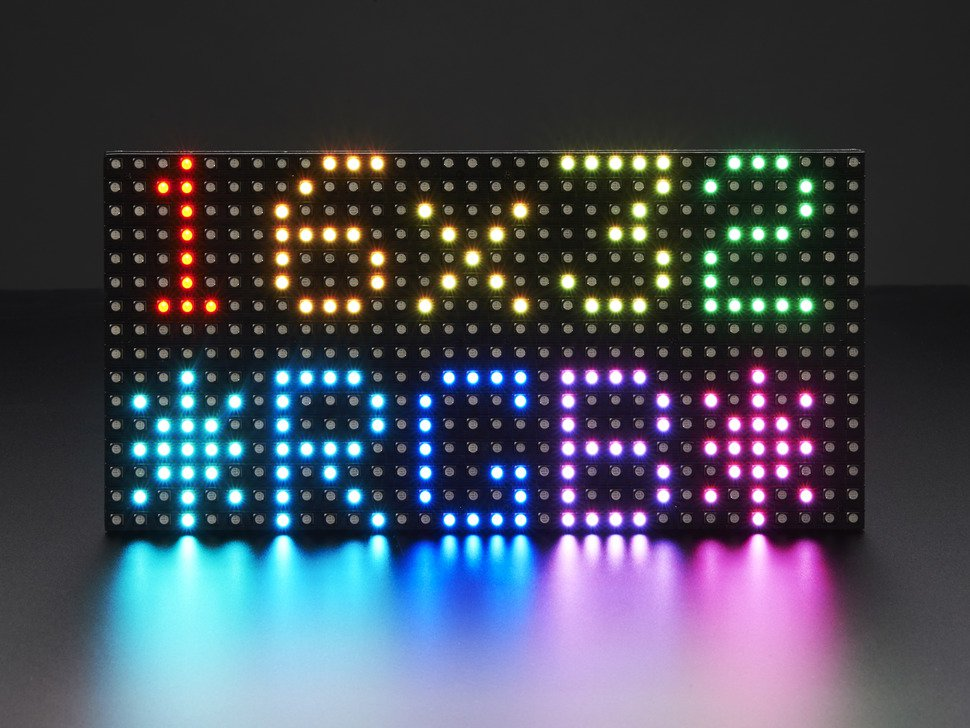
\includegraphics[scale=1]{RGBLEDMatrix.jpg}
	\caption{Verwendete LED-Matrix von Adafruit}
\end{figure}

Da die Matrix mit 16x32 deutlich über der Anforderung lag, wurde entschieden, dass auf der Matrix jeder Stein durch ein 2x2 Feld  dargestellt wird.
Das Feld würde somit eine Fläche von 12x14 einnehmen. Da somit immer noch genügend Platz vorhanden ist, und die Matrix mehr als zwei Farben anbietet, soll das Spielfeld durch einen Rand in einer anderen Farbe begrenzt werden.
Die somit ausgefüllte Fläche beträgt 14x16.
Zur besseren Visualisierung wurde zuletzt noch entschieden, über dem Spielfeld durch einen blinkenden Stein sowohl darzustellen, welcher Spieler aktuell am Zug ist, als auch in welche Spalte der nächste Stein aktuell gesetzt werden würde.
Insgesamt wird somit die Hälfte der Matrix genutzt, ein 16x16 Feld.
Aus ästhetischen Gründen wird daher das gesamte Feld in der Mitte der Matrix angezeigt.

\section{Ansteuerung der Matrix}
Zur Steuerung des Spielverlaufs ist ein Computer notwendig, welcher die Logik des 4 Gewinnt Spiels simulieren kann. Der Computer muss über 12 GPIO Pins zur Ansteuerung der LED-Matrix verfügen. Für diesen Zweck kommt ein \glqq Raspberry Pi 2 Model B\grqq{} zum Einsatz, welcher über 26 GPIOs Pins sowie weitere Pins für Masse und Stromversorgung verfügt.

\begin{figure}[!hbt]
	\centering
	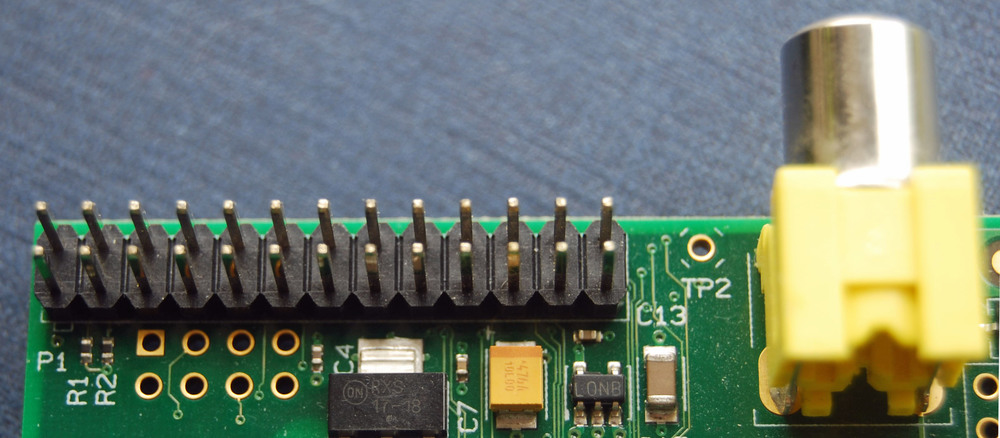
\includegraphics[scale=1]{gpio-pins}
	\caption{Nahaufnahme der Pins eines Raspberry Pis 2 Model B}
\end{figure}

Die GPIOs des Raspberry Pis werden mithilfe von mehreren Male/Female Jumpern mit der LED-Matrix verbunden. Um eine bessere Transportierbarkeit zu gewährleisten wird ein Aufsatz auf die GPIOs des Raspberry Pis verwendet. Die Verkabelung wird auf dem Aufsatz ausgeführt und dieser anschließend auf die GPIOs des Raspberry Pis gesteckt. Der Aufsatz ist abnehmbar und der Raspberry Pi somit unabhängig von der Verkabelung.

Für die Ansteuerung wird die Matrix ab der achten Zeile in zwei Hälften unterteilt. Beide Hälften können gleichzeitig angesteuert werden, um die Effizienz zu steigern. Um die darzustellende Farbe zu bestimmen sind je Hälfte 3 pins notwendig welche die RGB-Werte einer LED darstellen. Durch unterschiedliche Kombinationen der auf den Pins anliegenden Werte können die verschiedenen Farben auf den LEDs angezeigt werden. Weiter verfügt die Matrix über eine sogenannte \glqq clock \grqq{} mit der durch die einzelnen Spalten iteriert werden kann. Die \glqq clock \grqq{} wird dafür an einem GPIO des Raspberry Pis angeschlossen. Sobald ein Signal auf den Pin gelegt wird, wird die angesprochene LED um eine Spalte erhöht. Um die Zeile zu wählen werden 3 GPIO Pins angeschlossen. Diese stellen ein Binäres Signal zwischen 0 und 7 dar, welches die anzusprechende Zeile darstellt. Ein weiterer GPIO dient dabei als Signal um den Reihenwechsel zu initialisieren. Der verkabelte Aufbau kann in \refPicture{verkabelung} betrachtet werden.

\begin{figure}[!hbt]
	\centering
	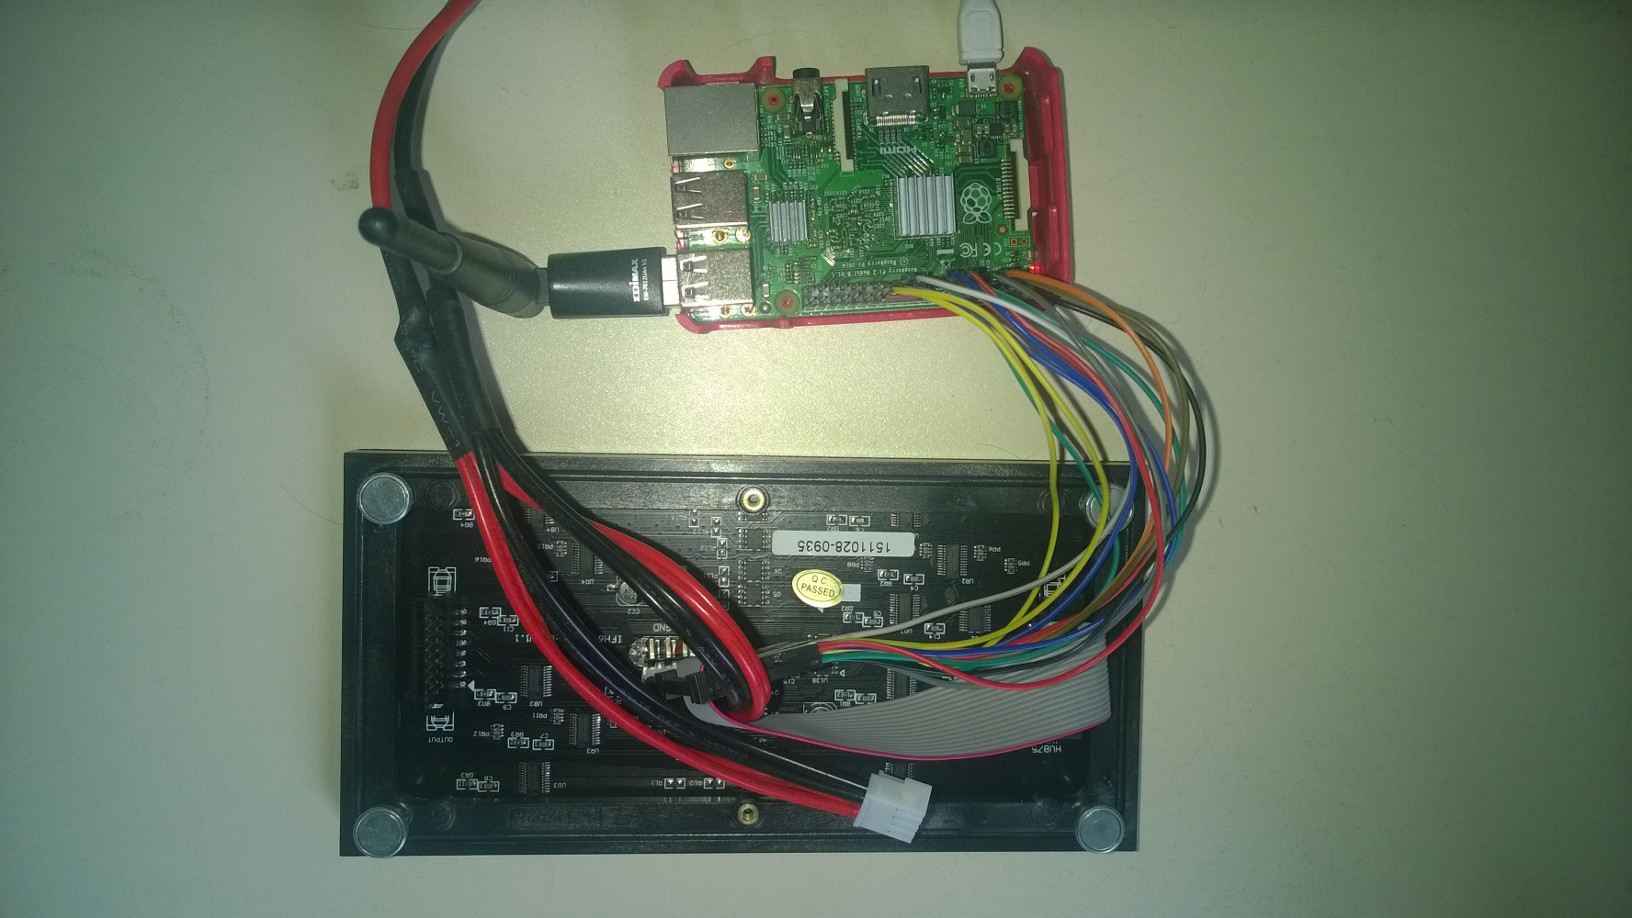
\includegraphics[scale=0.2]{Verkabelung}
	\caption{Verkabelung des Raspberry Pis und der LED-Matrix}
	\label{verkabelung}
\end{figure}

Das Programm wird mit der Programmiersprache Python entwickelt. Um die Signale auf die Pins des Raspberry Pis zu legen, kommt die Bibliothek RPi.GPIO zum Einsatz. Mithilfe der Bibliothek kann eine schnelle Ansteuerung der Pins erfolgen, die Signale können jedoch nur auf 0 oder 1 gelegt werden. Das hat zur Folge, dass die darzustellenden Farben deutlich eingeschränkt sind. Unter Angabe der Pinpositionen werden binäre Signale auf den Pins gelegt und die Matrix angesteuert.

\section{Umsetzung der 4 Gewinnt Logik}
Wie die Ansteuerung der Matrix erfolgt die Implementierung in Python. Die Klasse \textit{FourWins} dient zur Beschreibung des Spiels, stellt die Rahmenbedingungen fest und steuert den Spielverlauf. Innerhalb dieser Klasse wird sichergestellt, dass Spieler nacheinander ihre Züge machen, der Ablauf eines Zuges definiert und geprüft ist und ob das Spiel beendet wurde. \textit{FourWins} verfügt über eine 2-dimensionale Liste, welche das aktuelle Spielbrett darstellt. Die Einträge in der Liste stellen dabei den Spieler als kodierte Spielerfarbe dar. Sobald ein Spieler gewinnt werden die 4 gewinnenden Steine in grün eingetragen, um sie hervorzuheben

Das Spiel selbst wird durch die main-Funktion gesteuert. in der main-Funktion werden alternierend Spieler und Eingaben bestimmt, bis das Spiel beendet ist. Um zu setzende Spalte für den Spieler zu bestimmen wird ein temporärer Index genutzt. Diese gibt in welche Spalte der Stein hineingeworfen wird. Indem Tastatureingaben abgefangen werden wird diese Position nach rechts beziehungsweise links verschoben sollten rechte beziehungsweise linke Pfeiltaste gedrückt werden. Die zu setzende Spalte kann schließlich mit der Eingabe-Taste bestätigt werden. Weiter kann das Spiel jederzeit mit Betätigen der \glqq r \grqq -Taste zurückgesetzt und \glqq q \grqq -Taste beendet werden

Die Ansteuerung der GPIOs erfolgt über eine eigene Klasse. Dazu erhält es das Spielfeld von
\textit{FourWins} und stellt die darin liegenden Werte mittig in der LED-Matrix dar. Aufgrund der Größe der LED-Matrix wird jedem Wert zwei LEDs zugewiesen. Daraus entsteht eine neue 2-dimensionale Liste mit den Farbwerten für jede LED. Um das Spielfeld herum wird zusätzlich ein blauer Rahmen gelegt. Die dadurch entstandene Liste wird in hoher Frequenz auf der LED-Matrix neu gezeichnet, um ein stetiges Bild zu erzeugen. Aufgrund der mangelnden Echtzeitfähigkeit des Raspberry Pis kommt es hierbei jedoch zu einem leichten Flimmern. Um den Index der aktuell ausgewählten Spalte zu darzustellen wird ein neuer Thread verwendet. Dieser fügt in einem regelmäßigen Abstand einen Stein in Spielerfarbe über das Spielfeld, aber auf dem Index der Farbliste hinzu und löscht diesen nach einer Sekunde wieder. Dadurch entsteht wird der Index auf der Matrix durch einen blinkenden Stein in Spielerfarbe dargestellt

Das Spiel kann sowohl mit zwei menschlichen Spieler oder mit einem menschlichen Spieler und einer künstlichen Intelligenz gespielt werden.

\section{Künstliche Intelligenz}
Nachdem die Ansteuerung der Matrix mit Hilfe eines Python Skripts funktioniert, wurde noch eine Kümnstliche Intelligenz (KI) entwickelt, die anhand der gegebenen Informationen und Ressourcen in annehmbarer Zeit eine Zugentscheidung zu produzieren.
Wie in dem Kapitel \ref{sec:vierg} beschrieben handelt es sich bei \glqq Vier Gewinnt\grqq ~um ein Spiel mit perfekter Information handelt. Zusätzlich gehört das Spiel in die Kategorie der Nullsummenspiele. Dies bedeutet, dass die Gewinne und Verluste der beiden Spieler addiert stets 0 ergeben müssen.
Auf Grundlage dieser Informationen ist es möglich für eine KI den Minimax-Algorithmus einzusetzen.

Bei dem Minimax-Algorithmus handelt es sich um einen Gewinnoptimierungsalgorithmus, der über Heuristiken verschiedene Spielsituationen auswertet und den jeweilig besten Zug auswählt.
Für \glqq Vier Gewinnt\grqq ~muss der Algorithmus abgewandelt werden, da der Minimax-Algorithmus in seinen Grundzügen darauf optimiert ist einen maximierenden und einen minimierenden Spieler zu analysieren. Da bei \glqq Vier Gewinnt\grqq ~allerdings beide Spieler maximieren, muss bei der Analyse jeweils darauf geachtet werden, dass das Ergebnis des letzten Spielers negiert wird. Diese Abwandlung wird auch Negamax-Algorithmus genannt.

\begin{algorithm}
\caption{Negamax-Algorithmus}
\begin{algorithmic}[1]
\Procedure{NegaMax}{player, depth}
\If {$ depth == 0$~\textbf{or}~$\textit{noPlayableTurns}$} 
\State \Return $\textit{score(player)}$
\EndIf
\State $\textit{maxValue} \gets -\textit{infinity}$
\State $\textit{getPlayableTurns()}$
\While {$\textit{movableTurnsLeft}$}
\State $\textit{makeTurn()}$
\State $\textit{value} \gets -\textit{NegaMax(otherPlayer, depth-1)}$
\State $\textit{redoTurn()}$
\If {$\textit{value} \textgreater \textit{maxValue}$}
\State $\textit{maxValue} \gets \textit{value}$
\If {$\textit{depth} = \textit{requiredDepth}$}
\State $\textit{savedTurn} \gets \textit{turn}$
\EndIf
\EndIf
\EndWhile
\State \Return $\textit{maxValue}$
\EndProcedure
\end{algorithmic}
\end{algorithm}.